\chapter{Design-Time Network Performance Analysis of Distributed CPS Applications}
\label{ch:designTime}

In this chapter, we describe research contributions related to the
challenge of accurately predicting network QoS for systems which may
require strict guarantees about performance and resource utilization.

Many CPS applications require networking of some form in order for the
system to function nominally.  This networking often performs a key
role in the system, such as facilitating the communication and control
of distributed sensors and control systems.  Traditionally, these
networks of CPS have been both isolated from external influences and
predefined at system design-time.  This isolation and
pre-determination creates a static network with respect to both the
topology of the network and the capacity of each network link.  More
recently however, CPS have become less isolated and more dynamic by
utilizing heterogeneous and wireless networks and incorporating
mobility.  Such systems include wireless sensor networks (WSN), mobile
ad-hoc networks (MANETs), and distributed real-time embedded systems
(DRES).  These types of systems are being developed to provide remote
sensing and control capabilities, smart grid and smart city
infrastructure, and smart vehicle communications networks, to name a
few.

Analyzing application and system network Quality of Service (QoS)
requires either design-time models and analysis techniques or
experimental measurements from an application and system testbed.  For
high- or mixed-criticality software and systems, typically
experimental measurements are used but often these can be incomplete
or quite costly to generate.  Instead, a design-time modeling paradigm
for networked applications and systems can provide developers and
system integrators the information to accurately predict the system
and application network QoS.

Some wireless mobile CPS networks, such as the network between a
cluster of satellites orbiting Earth, vary periodically with respect
to time, \emph{e.g.} according to the cluster's orbital period.  For
such networks, the physical dynamics of the nodes in the cluster are
well understood and predictable, therefore the network dynamics can be
fairly predictable as well.  For such predictable or periodic dynamic
networks, the use of worst-case network performance for analysis and
constraint verification wastes the network resources over much of the
lifecycle of the system. Integrating the physical dynamics of the
network into the modeling and analysis tools improves the performance
of the systems without degrading its reliability.

To model the network capability of the system and the application
traffic patterns, we have developed a network modeling paradigm
similar to Network Calculus' traffic arrival curves and traffic shaper
service curves.  This paradigm is called \fulltool (\shorttool).  

Similarly to Network Calculus' arrival curves and service curves, our
network profiles model how the system's network performance or
application traffic generation changes with respect to time.  Whereas
Network Calculus' modeling transforms application data profiles and
network service profiles into max/min curves for data
received/serviced vs. length of time-window, our models take a simpler
approach which models exactly the data generated by the application
and the data which could be sent through the network, allowing our
performance metrics to be more precise.  Specifically, the bandwidth
that the network provides on a given communication link is specified
as a time series of scalar bandwidth values. Here, bandwidth is
defined as data rate, i.e. bits per second, over some averaging
interval.  This bandwidth profile can then be time-integrated to
determine the maximum amount of data throughput the network link could
provide over a given time.  The bandwidth profile for the application
traffic similarly can be time-integrated to determine the amount of
data that the application attempts to send on the network link as a
function of time.

We can use convolution ($\otimes$) between the application data
profile and the system network profile to obtain the transmitted link
data profile as a function of discrete time. The convolution we define
on these profiles borrows concepts from the min-plus calculus used in
Network Calculus. For a given application data generation profile,
$r[t]$, and a given system link capacity profile $p[t]$, where
$t\in\mathbb{N}$, the link transmitted data profile $l[t]$ is given by
the convolution Equation~\ref{eq:convolution}. The difference $(p[t-1]
- l[t-1])$ represents the difference between the amount of data that
has been transmitted on the link $(l[t-1])$ and the data that the link
could have transmitted at full utilization $(p[t-1])$. As demonstrated
by the convolution equation, $\forall t : l[t] \le r[t]$, meaning
without lower-layer reliable transport, the link cannot transmit more
application data for the application than the application requests.
Note that there will be packetization and communication header
overhead which will be transmitted with application data.  The
overhead can be determined at design time and can therefore be
accounted for in the application profile.

\begin{equation}
	\label{eq:convolution}
	\begin{split}
		y=l[t] &= (r \otimes p)[t] \\ &= min( r[t] , p[t] -
                (p[t-1] - l[t-1]) )
	\end{split}
\end{equation}
\vspace{-0.5in}
\begin{align}
	\label{eq:buffer}
	&\text{buffer}= sup\{r[t] - l[t] : t \in \mathbb{N}\}\\
	\label{eq:delay}
	&\text{delay} = sup\{l^{-1}[y]-r^{-1}[y] : y \in \mathbb{N}\}
\end{align}

\begin{figure}[h!]
	\centering
        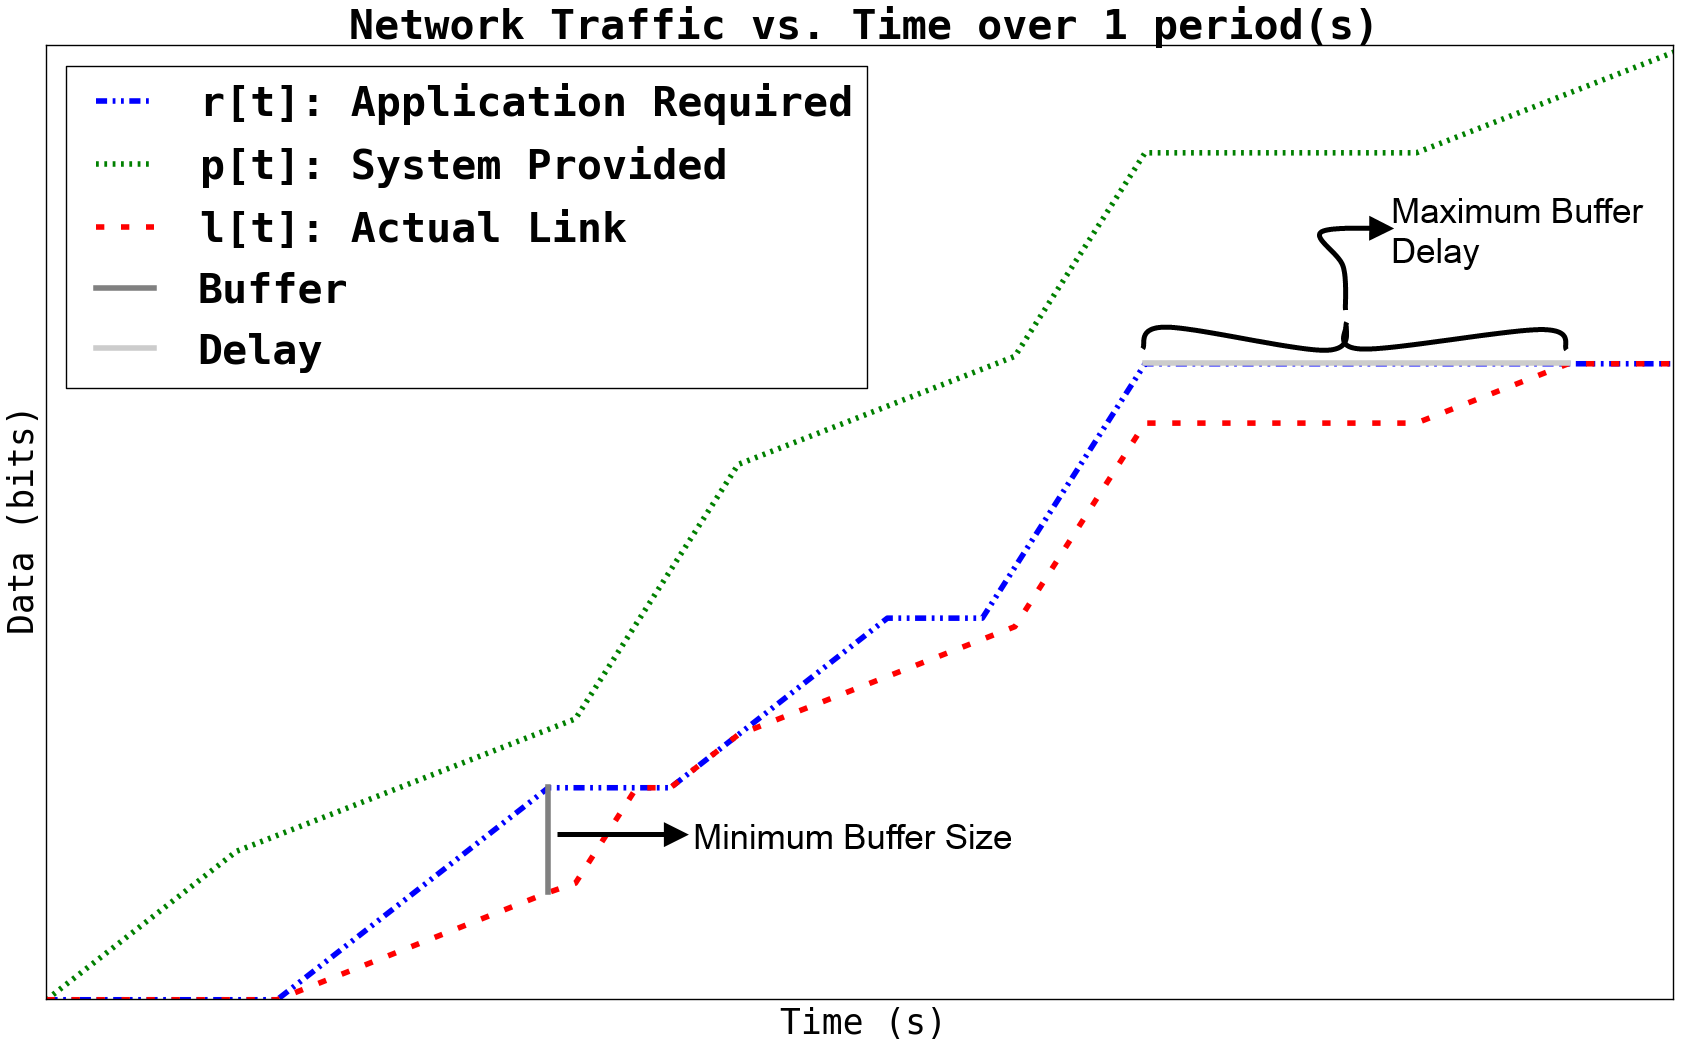
\includegraphics[width=0.85\textwidth]{figs/convolution6.png}
	\caption{Representative example demonstrating convolution of
          the data vs. time profiles that the application requires and
          that the system provides.  The resultant data vs. time
          profile describes the data that the system actually
          transmitted on the link.}
	\label{fig:convolution}
\end{figure}

Equation~\ref{eq:buffer} and Equation~\ref{eq:delay} calculate, using
$l[t]$, $r[t]$, and the inverse function $l^{-1}[y]$, the minimum
buffer size required for the application and the maximum buffering
delay experienced by application data, respectively.
Figure~\ref{fig:convolution} depicts the convolution operation and
shows a schematic representation of the maximum buffer delay and the
minimum buffer size.  As can be seen in the figure, the maximum
horizontal distance between the required profile and the link profile
is equal to the maximum buffer delay, while the maximum vertical
distance is equal to the minimum buffer size required for loss-less
transmission of data on the link.

\newpage
%%%%%%%%%%%%%%%%%%%%%%%%%%%%%%%%%%%%%%%%%%%%%%%%%%%%%%%%%%%%%%%%%%%%%%%%%%%%%%%%%%%
%%%%%%%%%%%%%%%%%%%%%%%%%%%%%%%%%%%%%%%%%%%%%%%%%%%%%%%%%%%%%%%%%%%%%%%%%%%%%%%%%%%
%%%%%%%%%%%%%%%%%%%%%%%%%%%%%%%%%%%%%%%%%%%%%%%%%%%%%%%%%%%%%%%%%%%%%%%%%%%%%%%%%%%
%%%%%%%%%%%%%%%%%%%%%%%%%%%%%%%%%%%%%%%%%%%%%%%%%%%%%%%%%%%%%%%%%%%%%%%%%%%%%%%%%%%
%%%%%%%%%%%%%%%%%%%%%%%%%%%%%%%%%%%%%%%%%%%%%%%%%%%%%%%%%%%%%%%%%%%%%%%%%%%%%%%%%%%
\section{Precise Modeling of Application Network Traffic and System Network Resources for Performance Prediction}
\label{sec:framework} 

To precisely predict network performance for applications distributed
in a mobile CPS, we need precise models of both the application
network resource requirements and the system's network resource
capacity.  These predictions, if precise and reliable enough, can
serve as guarantees for application developers and system integrators
about the network QoS that the system will provide and the network
resources the application will receive.

\subsection{Problem}
Current design tools do not incorporate the physical dynamics of the
network for analysis of network constraints on the
applications. Because of the diversity of CPS, IoT systems, and other
networked embedded systems in general, modeling and analysis tools
targeted towards these systems must support a wide range of
configurations, architectures, standards, and interfaces.  The same
compatibility is required in network modeling and analysis frameworks.
Because many of these systems may support different types of network
communications hardware, often using multiple types of network
interface hardware within the same system, the models of the network
must be able to express network resources in a way that can capture
these differences.  Because of this diversity and the modeling
semantics of the commonly used paradigms (e.g. Real-Time Calculus),
developing very precise predictions is difficult, since the models are
not very precise with respect to the actual behavior of the
applications on the system.

\subsection{Contributions}
\iffalse
\begin{itemize}
	\item We developed a network performance analysis technique,
          with associated system and application network resource
          models for wireless mobile CPS, reported in
          \cite{ISIS_F6_CYPHY:14}.
	\item We demonstrated how to compose the models together and
          derive application and system network performance metrics at
          design-time, reported in \cite{ISIS_F6_CYPHY:14}.
\end{itemize}
\fi

We developed the \shorttool paradigm, described above, to precisely
model system network resources as they vary with respect to time.
Similarly, the application network resource requirements can be
modeled very precisely as functions of time.  These models can be more
precise than the models developed for Network Calculus since they are
explicitly functions of time, instead of functions of time-windows.
Taking the example from earlier, a bulk data transfer (BDT) initiated
from the satellite cluster to a ground station is scheduled for when
the satellite cluster is within range of the ground station and
therefore has a good downlink to the ground.  With our paradigm, this
coupling between the network traffic flow and the network resource
availability can be captured explicitly in the model.  Under the
Network Calculus modeling semantics however, such a BDT would
negatively affect the predicted required network buffer size and
network buffering latency since that BDT data transmission window
(i.e. the window of time it sends the data on the link) would be
compared against the minimum service provided by the network to the
ground station (which would be zero during the parts of the orbit when
the ground stations are not within range of the cluster).  Such a
comparison drastically increases the predicted buffer space required
and predicted buffering latency incurred by the BDT data.

This network modeling and analysis technique we developed has been
reported in \cite{ISIS_F6_CYPHY:14}, which describes the network
resource models, their composition, and the calculation of performance
metrics such as buffer requirements and buffering delay.

\newpage
%%%%%%%%%%%%%%%%%%%%%%%%%%%%%%%%%%%%%%%%%%%%%%%%%%%%%%%%%%%%%%%%%%%%%%%%%%%%%%%%%%%
%%%%%%%%%%%%%%%%%%%%%%%%%%%%%%%%%%%%%%%%%%%%%%%%%%%%%%%%%%%%%%%%%%%%%%%%%%%%%%%%%%%
%%%%%%%%%%%%%%%%%%%%%%%%%%%%%%%%%%%%%%%%%%%%%%%%%%%%%%%%%%%%%%%%%%%%%%%%%%%%%%%%%%%
%%%%%%%%%%%%%%%%%%%%%%%%%%%%%%%%%%%%%%%%%%%%%%%%%%%%%%%%%%%%%%%%%%%%%%%%%%%%%%%%%%%
%%%%%%%%%%%%%%%%%%%%%%%%%%%%%%%%%%%%%%%%%%%%%%%%%%%%%%%%%%%%%%%%%%%%%%%%%%%%%%%%%%%
\section{Experimental Verification of Network Performance Prediction}
\label{sec:experimentalVerification}

\subsection{Problem}
When developing a new analysis technique to predict application
network performance, verification that the results of the analysis are
accurate is paramount.  Experimental results are required not only to
judge whether or not the theory is sound, but also to allow
application developers and system integrators to judge the
applicability of the analysis to their systems and applications.  If
the error in the predicted performance metrics is too high, the
analysis results will cease to be useful.

\subsection{Contributions}
We have developed a network emulation testbed which applies the
system's time-varying network profile to all network traffic in the
system, and has been reported in \cite{ISIS_F6_CYPHY:14}.  On this
testbed we ran application network traffic generation code which
produces network traffic according to the supplied application
profile.  This traffic generation code measured the delay, throughput,
and buffer requirements of the traffic that was generated.  By
collecting these measurements over the course of multiple tests, we
measured the differences between the predicted and measured buffer
size and delay.  The accuracy of our prediction was reported in
\cite{ISIS_F6_CYPHY:14}.

\newpage
%%%%%%%%%%%%%%%%%%%%%%%%%%%%%%%%%%%%%%%%%%%%%%%%%%%%%%%%%%%%%%%%%%%%%%%%%%%%%%%%%%%
%%%%%%%%%%%%%%%%%%%%%%%%%%%%%%%%%%%%%%%%%%%%%%%%%%%%%%%%%%%%%%%%%%%%%%%%%%%%%%%%%%%
%%%%%%%%%%%%%%%%%%%%%%%%%%%%%%%%%%%%%%%%%%%%%%%%%%%%%%%%%%%%%%%%%%%%%%%%%%%%%%%%%%%
%%%%%%%%%%%%%%%%%%%%%%%%%%%%%%%%%%%%%%%%%%%%%%%%%%%%%%%%%%%%%%%%%%%%%%%%%%%%%%%%%%%
%%%%%%%%%%%%%%%%%%%%%%%%%%%%%%%%%%%%%%%%%%%%%%%%%%%%%%%%%%%%%%%%%%%%%%%%%%%%%%%%%%%

\section{Point-to-Point TDMA Network Analysis}
\label{sec:tdma}

Medium channel access protocols are used in networking systems to
govern the communication between computing nodes which share a network
communications medium.  They are designed to allow reliable
communication between the nodes, while maintaining certain goals, such
as minimizing network collisions, maximizing bandwidth, or maximizing
the number of nodes the network can handle.  Such protocols include
Time Division Multiple Access (TDMA), which tries to minimize the
number of packet collisions; Frequency Division Multiple Access
(FDMA), which tries to maximize the bandwidth available to each
transmitter; and Code Division Multiple Access (CDMA) which tries to
maximize the number of nodes that the network can
handle\cite{jung1993advantagesCDMAFDMATDMA}.  We will not discuss CDMA
in the scope of this work.

In FDMA, each node of the network is assigned a different transmission
frequency from a prescribed frequency band allocated for system
communications.  Since each node transmits on its own frequency,
collisions between nodes transmitting simultaneously are reduced.
Communications paradigms of this type, i.e. shared medium with
collision-free simultaneous transmission between nodes, can be modeled
easily by our \shorttool modeling paradigm described above, since the
network resource model for each node can be developed without taking
into account the transmissions of other nodes.

In TDMA, each node on the network is assigned one or more time-slots
per communications period in which only that node is allowed to
transmit.  By governing these timeslots and having each node agree
upon the slot allocation and communications period, the protocol
ensures that at a given time, only a single node will be transmitting
data, minimizing the number of collisions due to multiple simultaneous
transmitters.  In such a medium access protocol, transmissions of each
node affect other nodes' transmission capability.  Because these
transmissions are scheduled by TDMA, they can be explicitly integrated
into the system network resource model.

\subsection{Problem}
TDMA transmission scheduling has an impact on the timing
characteristics of the applications' network communications.  Because
applications' network data production is decoupled from their node's
TDMA transmission time slot, buffering may be required when an
application on one node tries to send data on the network during the
transmission slot of a different node.  In this case, the data would
need to be buffered on the application's node and would therefore
incur additional buffering delay.  If this TDMA schedule is not
integrated into the analysis of the network resources, the additional
buffer space required may exceed the buffer space allocation given to
the application or the buffering delay may exceed the application's
acceptable latency.

\subsection{Contributions}
\iffalse
\begin{itemize}
	\item We extended our system and application network resource
          models to encompass TDMA based networks, reported in
          \cite{ISIS_F6_ISORC_QOS:15}.
	\item We derived formulas which abstracted away the TDMA
          scheduling to remove the requirement to explicitly
          incorporate the TDMA scheduling into the system and
          application models, reported in \cite{ISIS_F6_ISORC_QOS:15}.
\end{itemize}
\fi

We developed a model of TDMA in our \shorttool paradigm and analyzed
its affect on the performance metrics.  Through analysis of the
explicit TDMA schedule integrated into a system network resource
model, we were able to derive analytical formulas for the effect of
TDMA scheduling on application network buffering and delay.  We showed
how using these formulas removes the requirement for the explicit
integration of the TDMA schedule into the system network resource
model.  The TDMA modeling and analysis extension to our paradigm was
reported in \cite{ISIS_F6_ISORC_QOS:15}.

\newpage
%%%%%%%%%%%%%%%%%%%%%%%%%%%%%%%%%%%%%%%%%%%%%%%%%%%%%%%%%%%%%%%%%%%%%%%%%%%%%%%%%%%
%%%%%%%%%%%%%%%%%%%%%%%%%%%%%%%%%%%%%%%%%%%%%%%%%%%%%%%%%%%%%%%%%%%%%%%%%%%%%%%%%%%
%%%%%%%%%%%%%%%%%%%%%%%%%%%%%%%%%%%%%%%%%%%%%%%%%%%%%%%%%%%%%%%%%%%%%%%%%%%%%%%%%%%
%%%%%%%%%%%%%%%%%%%%%%%%%%%%%%%%%%%%%%%%%%%%%%%%%%%%%%%%%%%%%%%%%%%%%%%%%%%%%%%%%%%
%%%%%%%%%%%%%%%%%%%%%%%%%%%%%%%%%%%%%%%%%%%%%%%%%%%%%%%%%%%%%%%%%%%%%%%%%%%%%%%%%%%

\section{Network Performance Prediction Comparison with Other Analysis Tools}
\label{sec:comparison}

\subsection{Problem}
When developing a new analysis technique to predict application
network performance, alternative techniques must be evaluated to
determine the utility of the new techniques.  Application developers
and system integrators can then use these comparisons as a metric for
choosing between the available analysis tools.  For the tools and
techniques to affect a meaningful change in system and application
development, they must be shown to be more effective by some metric
for at least certain classes of systems or applications.

\subsection{Contributions}
\begin{itemize}
	\item We will develop test system and application models using
          our analysis techniques for which we can determine the
          predicted network resource requirements.
	\item We will develop those same test system and application
          models in RTC, using RTC Toolbox for MATLAB, for which we
          can determine comparison predicted network resource
          requirements.
	\item We will use our testbed to enforce the system profile
          and run application code which follows the network profile.
          Measurement code on the testbed and in the application will
          allow us to determine the application's network buffer
          utilization and buffering delay.
	\item We will compare the predicted results for the test
          system and application combinations to see what, if any,
          difference exists between the techniques.
\end{itemize}

\newpage
%%%%%%%%%%%%%%%%%%%%%%%%%%%%%%%%%%%%%%%%%%%%%%%%%%%%%%%%%%%%%%%%%%%%%%%%%%%%%%%%%%%
%%%%%%%%%%%%%%%%%%%%%%%%%%%%%%%%%%%%%%%%%%%%%%%%%%%%%%%%%%%%%%%%%%%%%%%%%%%%%%%%%%%
%%%%%%%%%%%%%%%%%%%%%%%%%%%%%%%%%%%%%%%%%%%%%%%%%%%%%%%%%%%%%%%%%%%%%%%%%%%%%%%%%%%
%%%%%%%%%%%%%%%%%%%%%%%%%%%%%%%%%%%%%%%%%%%%%%%%%%%%%%%%%%%%%%%%%%%%%%%%%%%%%%%%%%%
%%%%%%%%%%%%%%%%%%%%%%%%%%%%%%%%%%%%%%%%%%%%%%%%%%%%%%%%%%%%%%%%%%%%%%%%%%%%%%%%%%%

\section{Application Network Profile Generation from Business Logic Models}
\label{sec:generation}

Let us consider a platform that consists of a set of computing nodes,
each node equipped with a number of hardware devices. The nodes are
connected to each other over an ad-hoc, dynamic communication network.
We consider a subset of distributed software platforms, where the
applications are integrated from prefabricated components. A component
is the basic unit in the system that can provide a functionality. It
interacts with other components using well-defined interaction
patterns. Component-based software engineering has been extensively
applied to distributed real-time applications
~\cite{Emb_SW_PECOS:02,RT_CIAO:04,PROGRESS_ICSEA:08,ACM_SPE:10,ISIS_F6_ISORC:13}.

In this system, an application is essentially a group of components
that belong together and are typically deployed as a unit. A
middleware layer provides core communication abstractions such as
remote method invocation, asynchronous method invocation and
publish-subscribe interactions for the components. While additional,
more complex abstractions may also be needed, the interactions should
be facilitated in conjunction with overall system requirements. For
instance, the interactions can be subject to timing constraints, and
the scheduling of the message exchanges should be done accordingly.

When analyzing component-based software, models of the component
implementation (i.e. component models), allow compositional model
development.  Component models use the concepts of input/output
\emph{ports} to describe the interfaces through which a component
communicates with other components, which may be triggered by timers
or external events (e.g. the reception of data on a port).  Components
and component models are characterized by: (1) a specific set of
allowed component operations, (2) explicit scheduling paradigms for
those operations (e.g. first-in-first-out, FIFO), and (3) a specific
set of triggering events for component operations.  The components we
consider are single-threaded so each component in the system may only
perform a single operation at a time and will run that operation until
completion before starting the execution of the next operation.

The explicit restrictive nature of component-based software design
allows easier development of application behavior models which
describe the timing properties of each event or operation in the
application.  Because applications are broken down into components
whose execution is well defined, application developers can easily
model the behavior of the application by first modeling the behavior
of each port of each component.  This model of the behavior is called
the \textit{business logic model}, because it describes how the main
component code, the business logic of the component, behaves.
Captured in this model is the sequence of operations each port
performs, e.g. the timing, data production, and data consumption
involved with each port invocation.

We consider only applications with either finite execution time or
periodically repeating behavior.  Again we return to the satellite
cluster example presented earlier, which adheres to this model, as
both the system and its applications exhibit periodic behavior
according to the orbital period of the satellite cluster.

\subsection{Problem}
Developing an accurate, precise network resource requirement profile
for an application is a challenging and daunting task for all but the
simplest of applications.  Analysis of application network traffic to
determine worst-case data production over selected intervals
(e.g. every three minutes in a 90 minute periodic orbit) can provide a
better approximation of the network resource requirements than
traditional worst-case analysis over the entire lifetime of the
application.  However, this technique is not feasible for large or
complex applications and may yield only a marginal increase in model
fidelity.  Another possible technique for creating the application's
network resource requirement profile as a function of time is to run
the application on the target system with integrated measurement
facilities to more precisely and accurately determine the resource
requirements.  This technique however is impractical or infeasible for
application developers who do not have direct access to the system, or
for systems whose architectures or environments cannot be easily
simulated.

\subsection{Contributions}
\begin{itemize}
	\item We will develop an add-on to our currently existing
          modeling language for application business logic which
          captures the network resources required during each part of
          the business logic model.
	\item We will develop a compositional technique for generating
          the network resource requirement profile for an application
          from the combined business logic models of that
          application's components.  This is required because the
          business logic models describe the behavior of the callback
          associated with a component port, but does not describe the
          timing of the invocations of that callback.
	\item We will develop test applications for our testbed which
          adhere to the business logic models and allow us to measure
          the accuracy and precision of the predictions using these
          generated profiles.
\end{itemize}

\newpage
%%%%%%%%%%%%%%%%%%%%%%%%%%%%%%%%%%%%%%%%%%%%%%%%%%%%%%%%%%%%%%%%%%%%%%%%%%%%%%%%%%%
%%%%%%%%%%%%%%%%%%%%%%%%%%%%%%%%%%%%%%%%%%%%%%%%%%%%%%%%%%%%%%%%%%%%%%%%%%%%%%%%%%%
%%%%%%%%%%%%%%%%%%%%%%%%%%%%%%%%%%%%%%%%%%%%%%%%%%%%%%%%%%%%%%%%%%%%%%%%%%%%%%%%%%%
%%%%%%%%%%%%%%%%%%%%%%%%%%%%%%%%%%%%%%%%%%%%%%%%%%%%%%%%%%%%%%%%%%%%%%%%%%%%%%%%%%%
%%%%%%%%%%%%%%%%%%%%%%%%%%%%%%%%%%%%%%%%%%%%%%%%%%%%%%%%%%%%%%%%%%%%%%%%%%%%%%%%%%%

\section{Statically Routed Network Analysis}
\label{sec:staticRoute}

\subsection{Problem}
As CPS become more distributed in nature and begin to act as
infrastructure for distributed applications towards IoT systems, they
will necessarily need to handle more network resource management and
network connection routing within their network as well as between
their own network and any external networks to which they are
connected.  Such networks generally rely on routing to allow more
flexibility in the system with respect to node placement and
connectivity.  Adding routing to the network also has the effect of
increasing the complexity of the network performance analysis and can
cause drastic differences in application network performance when
compared with networks without routing.  Therefore the design-time
analysis tools which help predict application network performance must
take this routing into account.  It should be noted that this is a
special case of routing in ad-hoc networks, where one or more nodes
can route messages for other nodes.

\subsection{Contributions}
\begin{itemize}
	\item We will extend our network resource modeling and
          analysis techniques to support networks in which system
          nodes can act as routers for packets in the network.
	\item We will show experimentally the validity of the analysis
          results using our testbed and test applications.
\end{itemize}

\newpage
%%%%%%%%%%%%%%%%%%%%%%%%%%%%%%%%%%%%%%%%%%%%%%%%%%%%%%%%%%%%%%%%%%%%%%%%%%%%%%%%%%%
%%%%%%%%%%%%%%%%%%%%%%%%%%%%%%%%%%%%%%%%%%%%%%%%%%%%%%%%%%%%%%%%%%%%%%%%%%%%%%%%%%%
%%%%%%%%%%%%%%%%%%%%%%%%%%%%%%%%%%%%%%%%%%%%%%%%%%%%%%%%%%%%%%%%%%%%%%%%%%%%%%%%%%%
%%%%%%%%%%%%%%%%%%%%%%%%%%%%%%%%%%%%%%%%%%%%%%%%%%%%%%%%%%%%%%%%%%%%%%%%%%%%%%%%%%%
%%%%%%%%%%%%%%%%%%%%%%%%%%%%%%%%%%%%%%%%%%%%%%%%%%%%%%%%%%%%%%%%%%%%%%%%%%%%%%%%%%%

\section{Comparing \shorttool to Network Calculus}
\label{sec:equivalence}

\subsection{Problem}
Network Calculus has been around for a couple decades so far, and has
seen numerous improvements and extensions.  Mathematically analyzing
the equivalence between the methods of the proposed analysis with
those of Network Calculus would pave the way for enhancing the
proposed work with similar extensions as have been developed for
Network Calculus.  This equivalence analysis should hold, since both
techniques are based on the min-plus calculus dioid.  By showing the
equivalence, we would show that the proposed analysis techniques have
similar system-theory based applications.

\subsection{Contributions}
\begin{itemize}
	\item We will mathematically analyze the differences between
          the proposed technique and Network Calculus, showing that
          compositionality (i.e. concatenation of nodes in NC) applies
          to our analysis techniques
	\item We will analyze network flow composition to formalize
          operations for flow aggregation.
\end{itemize}
